\documentclass[11pt]{article}
\usepackage{mathpartir}
\usepackage{pifont}
\usepackage{multicol}
\usepackage{listings}
\usepackage{pgf}
\usepackage{tikz}
\usepackage{alltt}
\usepackage{hyperref}
\usepackage{url}
\usepackage{amsmath}
\usepackage{amssymb}
\usetikzlibrary{arrows,automata,shapes,positioning}
\tikzstyle{block} = [rectangle, draw, fill=blue!20, 
    text width=5em, text centered, rounded corners, minimum height=2em]
\tikzstyle{bt} = [rectangle, draw, fill=blue!20, 
    text width=1em, text centered, rounded corners, minimum height=2em]
\newcommand{\xmark}{\ding{55}}

\newtheorem{defn}{Definition}
\newtheorem{crit}{Criterion}
\newcommand{\true}{\mbox{\sf true}}
\newcommand{\false}{\mbox{\sf false}}

\newcommand*\circled[1]{\tikz[baseline=(char.base)]{
            \node[shape=circle,draw,inner sep=2pt] (char) {#1};}}


\newcommand{\handout}[5]{
  \noindent
  \begin{center}
  \framebox{
    \vbox{
      \hbox to 5.78in { {\bf Software Testing, Quality Assurance and Maintenance } \hfill #2 }
      \vspace{4mm}
      \hbox to 5.78in { {\Large \hfill #5  \hfill} }
      \vspace{2mm}
      \hbox to 5.78in { {\em #3 \hfill #4} }
    }
  }
  \end{center}
  \vspace*{4mm}
}

\newcommand{\lecture}[4]{\handout{#1}{#2}{#3}{#4}{Lecture #1}}
\topmargin 0pt
\advance \topmargin by -\headheight
\advance \topmargin by -\headsep
\textheight 8.9in
\oddsidemargin 0pt
\evensidemargin \oddsidemargin
\marginparwidth 0.5in
\textwidth 6.5in

\parindent 0in
\parskip 1.5ex
%\renewcommand{\baselinestretch}{1.25}

\usepackage{enumitem}

\newtheorem{prop}{Proposition}
\newtheorem{lemma}{Lemma}
\usepackage{ebproof}
\newcommand{\qedsymbol}{\rule{1ex}{1ex}}
\newcommand{\sem}[3]{\langle #1, #2 \rangle \Downarrow #3}

\lstset{ %
language=Java,
basicstyle=\ttfamily,commentstyle=\scriptsize\itshape,showstringspaces=false,breaklines=true,numbers=left}

%\usepackage{fontspec}
%\setmonofont{Cousine}[Scale=MatchLowercase]

\begin{document}

\lecture{12 --- February 26, 2025}{Winter 2025}{Patrick Lam}{version 1}

We've seen this picture on the slides.

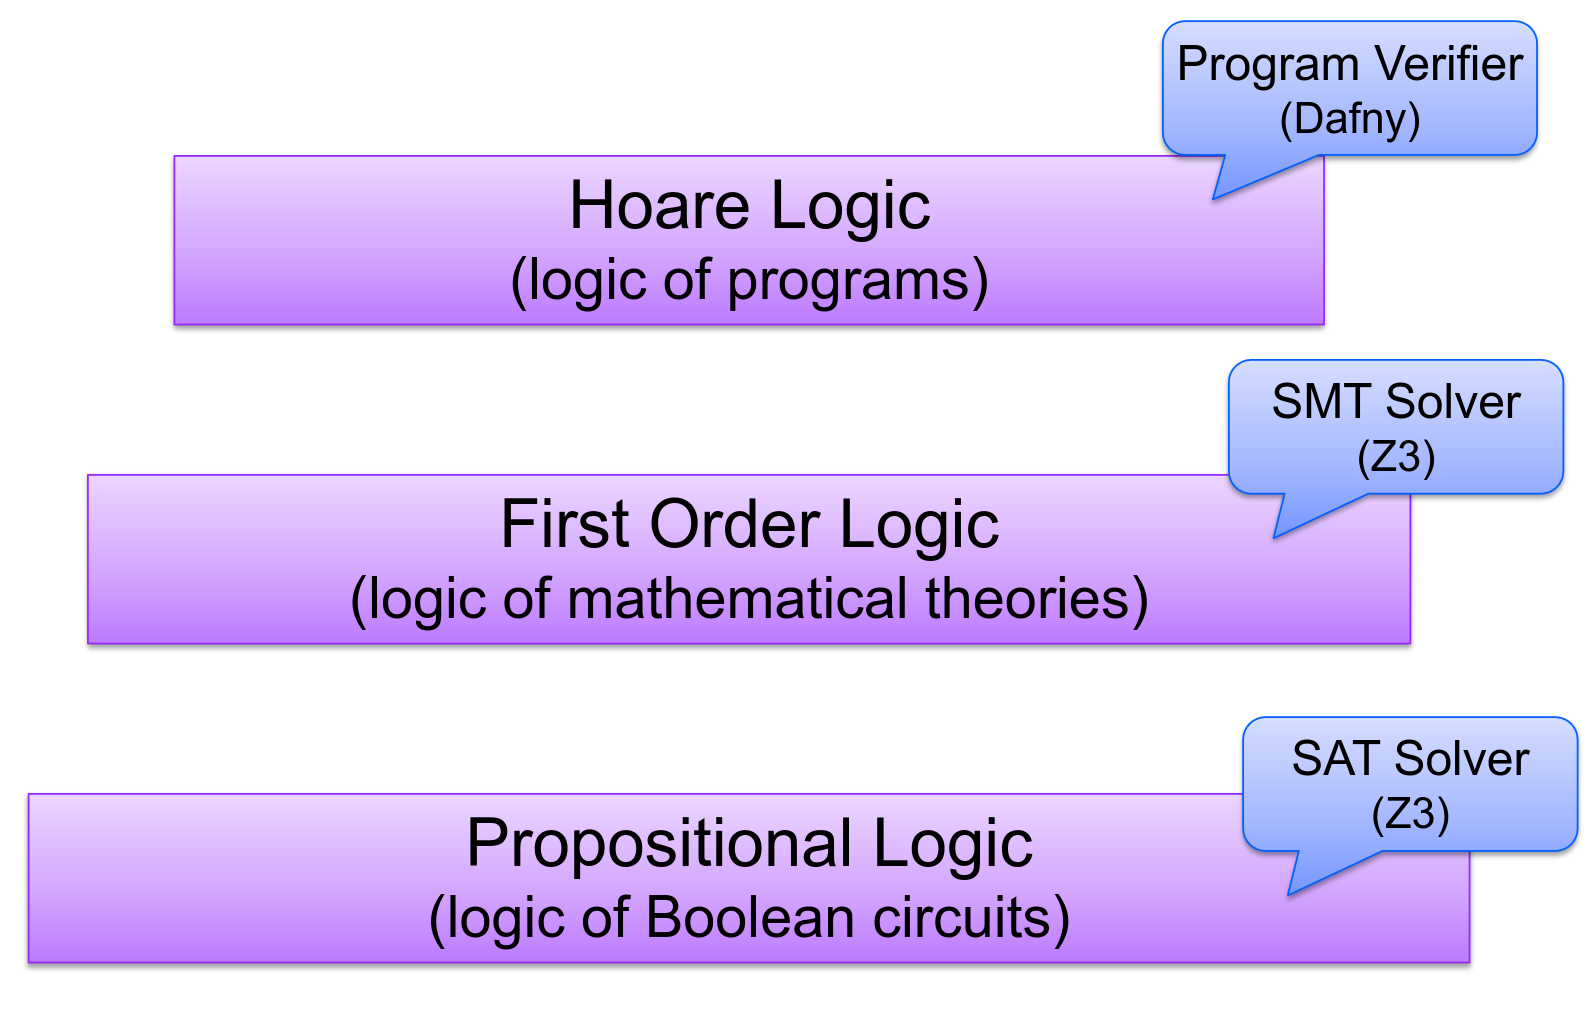
\includegraphics[width=\textwidth]{L12/three-logics.png}

This lecture is about Hoare Logic. Again, you've seen this in SE 212, but it's worth a review as we
prepare to move onto Dafny. Some of the concepts are subtle!

%https://www.site.uottawa.ca/~afelty/csi5137/plf/Hoare.html
%https://cs.stackexchange.com/questions/118322/why-is-the-assignment-rule-the-way-it-is-in-hoare-logic
%https://www.cs.cornell.edu/courses/cs4160/2019sp/terse/plf/Hoare.html

\paragraph{Axiomatic Semantics.} You used axiomatic semantics in SE 212.
It consists of:
\begin{itemize}[noitemsep]
\item a language for stating assertions about programs; and
  \item rules for establishing the truth of assertions.
\end{itemize}

You have used axiomatic semantics to make and prove assertions. Some examples:
\begin{itemize}[noitemsep]
\item this program terminates;
\item if this program terminates, the variables \texttt{x} and \texttt{y} have the same value throughout the execution of the program;
\item array accesses are within array bounds.
\end{itemize}

One can use first-order logic for assertions. There are also
special-purpose specification languages, which I'll name-check but not
discuss: Z (the OG specification language), Larch, JML.  And there are
other logics as well: temporal logic, especially useful for specifying
properties of concurrent systems; linear logic, which has been used
under-the-hood for Rust uniqueness; and separation logic, for
reasoning about the structure of the heap.

\paragraph{Hoare Triples.} We write assertions about WHILE programs using Hoare triples:
\[ \{ A \} ~c~ \{ B \} \]
which means that (1) if $A$ holds in state $q$, and (2) if the semantics says $q \rightarrow q'$, then (3) $B$ holds in $q'$.

One can thus write the valid assertion
\[ \{ y \leq x \} z := x; z := z + 1 \{ y < z \} \]
which means that if $y \leq x$ and you run those two statements, you know that $y < z$ at the end of them.

\paragraph{Partial versus total correctness.} More specifically, $\{A\} ~c~ \{ B\}$ is a \emph{partial} correctness assertion,
and does not imply termination of $c$.

If $A$ holds in state $q$, and if there exists $q'$ such that $q \rightarrow q'$, then $B$ holds in state $q'$. So,
if there is no $q'$ (i.e. $c$ does not terminate, or gets stuck), then there is, vacuously, no obligation to show $B$.

There is the notion of \emph{total} correctness as well, though much less often used. $[A] ~c~ [B]$ is the notation for
\emph{total} correctness.

If $A$ holds in state $q$, {\bf then} there exists $q'$ such that $q \rightarrow q'$, and $B$ holds in state $q'$.

\subsection*{More formal Hoare logic}
We have assertions like $A$ and $B$. We'll formalize the language we use for them,
define when an assertion holds in a state, and define rules for deriving valid Hoare triples.

\paragraph{Our assertion language.}
We use \emph{first-order predicate logic} and use WHILE expressions as atoms.

\begin{eqnarray*}
  A &::==& \mathsf{true} \mid \mathsf{false} \mid e_1 = e_2 \mid e_1 \geq e_2 \\
  &\mid& A_1 \wedge A_2 \mid A_1 \vee A_2 \mid A_1 \Rightarrow A_2 \mid \forall x. A \mid \exists x. A
\end{eqnarray*}
There are logical variables (e.g. $\forall x$) and program variables.
We don't distinguish them. For our purpose, all WHILE variables range over integers.

It is always valid to use a WHILE Boolean expression as an assertion.

\paragraph{Semantics of assertions.}
We write
\[ q \models A \]
to mean that assertion $A$ holds in state $q$.
(It is well-defined when $q$ is defined on all variables occuring free in $A$).

We define $\models$ inductively on the structure of assertions. (Start with the atomic assertions
and arithmetic expressions from WHILE, and then build up the compound assertions like $\wedge$ etc.)

\[
\begin{array}{ll}
  q \models \mathsf{true} & \mbox{always} \\
  q \models e_1 = e_2 &    \mbox{iff~} \sem{e_1}{q}{}~ = \sem{e_2}{q}{} \\
  q \models e_1 \geq e_2 & \mbox{iff~} \sem{e_1}{q}{}~ \geq \sem{e_2}{q}{} \\
  q \models A_1 \wedge A_2 & \mbox{iff~} q \models A_1 \mathrm{~and~} q \models A_2 \\
  q \models A_1 \vee A_2 & \mbox{iff~} q \models A_1 \mathrm{~or~} q \models A_2 \\
  q \models A_1 \Rightarrow A_2 & \mbox{iff~} q \models A_1 \mathrm{~implies~} q \models A_2 \\
  q \models \forall x.~ A & \mbox{iff~} \forall n \in \mathbb{Z}.~q[x:=n] \models A\\
  q \models \exists x.~ A & \mbox{iff~} \exists n \in \mathbb{Z}.~q[x:=n] \models A\\
\end{array}
\]

\paragraph{Semantics of Hoare Triples.} In symbols, then, partial correctness means:
\begin{eqnarray*} && \models \{ A \} ~c~ \{ B \} \mbox{ iff } \\
  && \qquad \forall q, q' \in Q.~ q \models A \wedge q \xrightarrow{c} q' \Rightarrow q' \models B
\end{eqnarray*}
Total correctness means:
\begin{eqnarray*} && \models [ A ] ~c~ [ B ] \mbox{ iff } \\
  && \qquad \forall q \in Q.~ q \models A \Rightarrow \exists q' \in Q.~ q \xrightarrow{c} q' \wedge q' \models B
\end{eqnarray*}
Quantifier selection matters!

\paragraph{Examples of Hoare Triples.} Let's fill in the blanks for these Hoare triples. I'll put the blank versions first.

\[
\begin{array}{lll}
  \{ \mathsf{~true~} \} & x := 5 &\{ \hspace*{5em} \} \\
  \{ \hspace*{5em} \} & x := x + 3 &\{ x = y + 3 \} \\
  \{ \hspace*{5em} \} & x := x * 2 + 3 &\{ x > 1 \} \\
  \{ x = a \} & \mathsf{if~} x < 0 \mathsf{~then~} x := -x  &\{ \hspace*{5em} \} \\
  \{ \mathsf{~false~} \} & x := 3  &\{ \hspace*{5em} \} \\
  \{ x > 0 \} & \mathsf{while~} x \mathtt{!=~} 0 \mathsf{~do~} x := x - 1  &\{ \hspace*{5em} \} \\
  \{ x > 0 \} & \mathsf{while~} x \mathtt{!=~} 0 \mathsf{~do~} x := x - 1 & \{ \hspace*{5em} \} \\
\end{array}
\]

You can find the solutions at the end of this document.

\section*{Inference rules}

We do now have a definition for $\{A\} ~c~ \{B\}$. But the definition
relies heavily on having $q \xrightarrow{c} q'$, which is defined by
the operational semantics. This is inconvenient: we pretty much have
to run the program to verify an assertion. And it's even harder when
there are loops.  And, if you want to verify $\forall x.~A$, you have
to run the program for all possible $x$, which is hard.

This is why you used inference rules and the axiomatic semantics in SE 212.
We can symbolically verify assertions without running the program.

\subsection*{Inference rules for First-Order Logic.} The notation $\vdash A$ means that
$A$ can be inferred from the axioms. $B \vdash A$ means that $A$ can be inferred from $B$.

We are going to use natural deduction style rules. Substitution is always confusing,
so as a reminder, $A[a/x]$ means $A$ with variable $x$ replaced by term $a$ (``substitute $a$ for $x$'').

\begin{center}
  \begin{tabular}{ccc}
  $\inferrule*{A ~~~~ B }{A \wedge B}$ &
  $\inferrule*{A}{A \vee B} \hspace*{1em} \inferrule*{B}{A \vee B}$ &
  $\inferrule*{A \rightarrow B \hspace*{2em} A}{B}$\\[2em]

  $\inferrule*{A[e/x]}{\exists x. A}$ &
  $\inferrule*{\forall x.~A}{A[e/x]}$ &
  $\inferrule*[Right=$a \mathrm{~fresh}$]{A[a/x]}{\forall x.~A}$\\[2em]
  
  $\inferrule*{A \vdash B}{A \Rightarrow B}$ &
  \multicolumn{2}{c}{$\inferrule*[Right=$a \mathrm{~fresh}$]{\vdash \exists x.~A ~~~~ A[a/x] \vdash B}{\vdash B}$}
  \end{tabular}
\end{center}

\subsection*{Inference rules for Hoare triples} We write $\vdash \{A\}~c~\{B\}$ when we can derive
the triple using inference rules.

There is one inference rule for each command in WHILE.

\paragraph{Rule of Consequence.} It is also always allowed to strengthen the pre-condition or weaken the post-condition.

\[
\inferrule*[Right=\textsc{Conseq}]{\vdash A' \Rightarrow A ~~~~ \{A\}~c~\{B\}~~~~ \vdash B \Rightarrow B'}{\{A'\}~c~\{B'\}}
\]

For example, let's look at this Hoare triple.
\[ \{ x = 2 \} ~ \texttt{x := 5}~ \{ x = 5 \} \]

Can we weaken the precondition? That is, are there other pre-states where executing \texttt{x := 5} will still result in postcondition
$x=5$? Yep. If we start with precondition $ x = 19$ and run \texttt{x := 5} we still get postcondition $x=5$. Indeed, in \emph{any} pre-state,
running \texttt{x := 5} results in $x=5$ being true.

So, the weakest possible precondition here is \textsf{true}, and we generally want to put the weakest precondition that we can---the one that restricts
allowable states least.
\[ \{ \mathsf{true} \} ~ \texttt{x := 5}~ \{ x = 5 \} \]

What about strengthening the postcondition? Let's look now at this Hoare triple.

\[ \{ \mathsf{true} \} ~ \texttt{x := 5}~ \{ \mathsf{true} \} \]

This isn't saying anything useful. It is saying that you can execute \texttt{x := 5} in any state, and you know nothing (``true'') after running it.
No matter what happens, this Hoare triple is going to be valid.

Consider instead
\[ \{ \mathsf{true} \} ~ \texttt{x := 5}~ \{ x > 0 \} \]
This is still valid, and it's slightly more useful---a stronger postcondition, which restricts possible states more.
The strongest (most restrictive) postcondition, which tells you the most about what this statement is doing, is
what we had before, 
\[ \{ \mathsf{true} \} ~ \texttt{x := 5}~ \{ x = 5 \} \]

\paragraph{The Rules.} Here they are.

\begin{center}
  \begin{tabular}{cc}
  \{A\}~\texttt{skip}~\{A\} &
  \inferrule{\{A\}~s_1~\{B\} ~~ \{B\}~s_2~\{C\}}{\{A\}~s_1 \texttt{~;~} s_2~~\{C\}}  \\[2em]

    \{A[e/x]\}~\texttt{x := e}~\{A\} &
  \inferrule{\{A \wedge b\}~s_1~\{B\} ~~ \{A \wedge \neg b\}~s_2~\{B\}}{\{A\}~\texttt{if $b$ then $s_1$ else $s_2$}~~\{B\}}  \\[2em]

  \multicolumn{2}{c}{
    \inferrule{\{I \wedge b\}~s~\{I\} }{\{I\}~\texttt{while $b$ do $s$}~~\{I \wedge \neg b\}}
    }
  \end{tabular}
\end{center}

\paragraph{About that Assignment Rule.} It is, yes, a bit surprising. Why is it backwards-looking?
\[
\{A[e/x]\}~\texttt{x := e}~\{A\}
\]
In the semantics, the rules always went from a state $q$ to its successor $q'$ (even if sometimes we worked backwards in writing derivations).
One way to think about this assignment rule is that you have the postcondition $A$. The rule tells us what is the weakest
poscondition that we can write such that, after executing assignment \texttt{x := e}, we have postcondition $A$.

So, what about
\[
\{ \hspace*{4em} \} ~\texttt{x := y}~ \{ x = 1 \}
\]
Here, we are given postcondition $\mathtt{x} = 1$. The assignment statement copies the value from \texttt{y} into \texttt{x}.
Thus, the weakest precondition yielding the given postcondition is
\[
\{ y = 1 \} ~\texttt{x := y}~ \{ x = 1 \}
\]
We can interpret this Hoare triple as: if \texttt{y} starts with value 1 and we copy that value into \texttt{x}, then we know
\texttt{x} finishes with value 1. This is the weakest precondition because any other value of \texttt{y} is not going to yield
$x = 1$ at the end. The triple, in general, transfers the property of being 1 from \texttt{y} to \texttt{x}.

Now, let $y+z$ be equal to 1 in the precondition
\[
\{ y+z = 1 \} ~\texttt{x := y+z}~ \{ ? \}
\]
Then, the strongest postcondition has $x$ being equal to 1 (though you are allowed to say less).
\[
\{ y+z = 1 \} ~\texttt{x := y+z}~ \{ x = 1 \}
\]

Let's generalize a bit more.
\[
\{ a = 1 \} ~\texttt{x := a}~ \{ x = 1 \}
\]
We are still transferring the 1 from expression $a$ (it doesn't have to be a variable, it's logic) to $x$.

And finally, we can get the full assignment rule
\[
\{A[e/x]\}~\texttt{x := e}~\{A\}
\]
We get to state $A$ after assignment \texttt{x := e} if we had started, in the precondition, with a state like $A$ except with term $e$ in the precondition instead of the $x$ we have in the postcondition.
(It is actually allowed to replace any number of $x$s in the postcondition, including 0, to form the precondition.)

Here is an example.
\[
\{x \leq 5[x+1/x]\}~\texttt{x := x + 1}~\{ x \leq 5\}
\]
Doing the substitution, we have
\[
\{x+1 \leq 5\}~\texttt{x := x + 1}~\{ x \leq 5\}
\]
which is the weakest possible precondition that gives you $x \leq 5$ as postcondition.

\paragraph{Example: Conditional} We deduce a postcondition that is true no matter which branch of the conditional we take.

\[
\begin{prooftree}
  \hypo{D_1:: \{ \mathsf{true} \wedge y \leq 0 \} ~ \texttt{x := 1} ~ \{ x > 0 \}}
  \hypo{D_2:: \{ \mathsf{true} \wedge y > 0 \} ~ \texttt{x := y} ~ \{ x > 0 \}}
  \infer2{ \{ \mathsf{true} \} \mathsf{~if~} y \leq 0 \mathsf{~then~} x := 1 \mathsf{~else~} x := y ~ \{ x > 0 \}}
\end{prooftree}
\]

We can deduce $D_1$ by the rules of consequence and assignment. In particular, we strengthen the precondition
for the rule of assignment.
\[
\begin{prooftree}
  \hypo{\mathsf{true} \wedge y \leq 0 \Rightarrow 1 > 0}
  \hypo{\{ 1 > 0 \} ~ \texttt{x := 1} ~ \{ x > 0 \}}
  \infer2{\{ \mathsf{true} \wedge y \leq 0 \} ~ \texttt{x := 1} ~ \{ x > 0 \}}
\end{prooftree}
\]
Similarly for $D_2$:
\[
\begin{prooftree}
  \hypo{\mathsf{true} \wedge y > 0 \Rightarrow y > 0}
  \hypo{\{ y > 0 \} ~ \texttt{x := y} ~ \{ x > 0 \}}
  \infer2{\{ \mathsf{true} \wedge y > 0 \} ~ \texttt{x := y} ~ \{ x > 0 \}}
\end{prooftree}
\]

\paragraph{Exercise: Alternative Assignment Rule.} Is this rule correct?

\[ \vdash \{ \mathsf{true} \}~ \texttt{x := e} ~ \{ x = e \} \]

It's appealing, but no. If we used that rule, then we could deduce the following incorrect
Hoare triple.

\[ \vdash \{ \mathsf{true} \}~ \texttt{x := x + 1} ~ \{ x = x + 1 \} \]

which boils down to postcondition $0 = 1$, or \textsf{false}, which isn't useful.

\paragraph{Actually correct alternative rules.} We can actually use this axiom for assignment:

\[
\vdash \{ A \}~ \texttt{x := e} ~ \{ \exists x_0. \texttt{x = e}[x_0/x] \wedge A[x_0/x] \} \]
In some sense, it is creating a copy of $e$ with the original $x$ substituted by fresh $x_0$, setting $x$ to that copy, and
also substituting the same fresh $x_0$ into $A$ in place of $x$.

For while loops, we could use:
\[
\begin{prooftree}
\hypo{\vdash I \wedge b \Rightarrow C}
\hypo{\{ C \} ~c~ \{ I \}}
\hypo{\vdash I \wedge \neg b \Rightarrow B}
\infer3{\vdash \{I\} ~\texttt{while $b$ do $c$}~\{C\}}
\end{prooftree}
\]
These rules are derivable from the previous rules plus the rule of consequence.

\paragraph{Example: a simple loop.}
We want to infer the Hoare triple
\[ \{ x \leq 0 \} \texttt{~while $x \leq 5$ do $x := x + 1$~}  \{ x=6\} \]
which says that, starting with $x$ not positive, incrementing it while $x \leq 5$ results in final state $x = 6$.

We choose loop invariant $I: x \leq 6$ and use the while and assignment rules, along with the rule of consequence.

\[
\begin{prooftree}
  \hypo{x \leq 6 \wedge x \leq 5 \Rightarrow x + 1 \leq 6}
  \hypo{\{ x+1 \leq 6 \} ~\texttt{x := x + 1}~ \{ x \leq 6 \}}
  \infer2{\{ x \leq 6 \wedge x \leq 5\} ~\texttt{x := x + 1}~ \{ x \leq 6 \}}
  \infer1{\{ x \leq 6\} ~\texttt{while x <= 5 do x := x + 1}~ \{ x \leq 6 \wedge x > 5 \}}
\end{prooftree}
\]
We finally apply the rule of consequence.
\[
\begin{prooftree}
  \hypo{x \leq 0 \Rightarrow x \leq 6}
  \hypo{x \leq 6 \wedge x > 5 \Rightarrow x = 6}
  \hypo{\{x \leq 6\} ~\texttt{while \ldots}~ \{ x \leq 6 \wedge x > 5\} }
  \infer3{\{x \leq 0\} ~\texttt{while x <= 5 do x := x + 1}~\{ x = 6 \}}
\end{prooftree}
\]

\paragraph{Inductive Loop Invariants.} Here is another concept that you've seen before in SE 212, but which is
well worth repeating, as you'll need this to use Dafny.

We want to be able to reason about loops without having to unroll the loop an unbounded number of times.
The key is to find a \emph{loop invariant} which is true no matter how many times the loop executes.
Then we show that the loop invariant holds upon entry to the loop and is preserved by the loop body.
We also need to show that it is strong enough to show what we need after the loop. Also, inside the loop,
we know that the loop condition holds (that's why we're inside the loop), and upon exit from the loop,
the negation of the loop condition holds (which allows us to exit).

\[
\begin{prooftree}
  \hypo{\mathrm{Pre} \Rightarrow \mathrm{Inv}}
  \hypo{\{ \mathrm{Inv} \wedge b \} ~s~ \{ \mathrm{Inv} \}}
  \hypo{\{ \mathrm{Inv} \wedge \neg b \} ~s~ \{ \mathrm{Post} \}}
  \infer3{\{ \mathrm{Pre} \} ~\texttt{while $b$ do $s$}~ \{ \mathrm{Post} \}}
\end{prooftree}
\]

Specifically, Inv is an \emph{inductive loop invariant} if the following three conditions holdD:
\begin{itemize}[noitemsep]
\item (Initiation): Inv holds \emph{initially} whenever the loop is reached; i.e. the pre-condition of the loop, Pre,
  implies Inv.
\item (Consecution): Inv is \emph{preserved}: if $\mathrm{Inv} \wedge b$ holds before executing the loop body, then executing all the statements in the loop body will end in a state that also satisfies Inv.
\item (Safety): $\mathrm{Inv} \wedge \neg b$ implies the desired postcondition Post.
\end{itemize}

\paragraph{Simple Loop using Inductive Invariants.} Consider again the loop:
\[ \{ x \leq 0 \} \texttt{~while $x \leq 5$ do $x := x + 1$~}  \{ x=6\} \]
but now we use inductive invariant $x \leq 6$. One application of the inductive invariant rule above:
\[
\begin{prooftree}
  \hypo{x \leq 0 \Rightarrow x \leq 6}
  \hypo{\{ x \leq 7 \wedge x \leq 5 \} ~\texttt{x := x + 1}~ \{ x \leq 6 \}}
  \hypo{x > 5 \wedge x \leq 6 \Rightarrow x = 6}
  \infer3{\{ x \leq 0\}\texttt{~while $x \leq 5$ do $x := x + 1$~}  \{ x=6\}}
\end{prooftree}
\]

\paragraph{Completed Hoare triples.} These are the strongest postconditions / weakest preconditions from before.

\[
\begin{array}{lll}
  \{ \mathsf{~true~} \} & x := 5 &\{ x = 5 \} \\
  \{ x = y \} & x := x + 3 &\{ x = y + 3 \} \\
  \{ x * 2 > -1 \} & x := x * 2 + 3 &\{ x > 1 \} \\
  \{ x = a \} & \mathsf{if~} x < 0 \mathsf{~then~} x := -x  &\{ x \leq 0 \Rightarrow x = -a ~\wedge~ x > 0 \Rightarrow x = a \} \\
  \{ \mathsf{~false~} \} & x := 3  &\{ \mathsf{~true~} \} \\
  \{ x > 0 \} & \mathsf{while~} x \mathtt{!=~} 0 \mathsf{~do~} x := x - 1  &\{ x = 0 \} \\
  \{ x > 0 \} & \mathsf{while~} x \mathtt{!=~} 0 \mathsf{~do~} x := x - 1 & \{ \mathsf{~true~} \} \\
\end{array}
\]

\end{document}
